As shown in Figure~\ref{fig:abla_llama}, 
\hero with \llama as bacnkbone demonstrate similar trends with \hero-Qwen, exceot MusiQue and Bamboogle. Prompt Evolution is the most critical component. Its removal results in the largest drops across nearly all datasets. For example, F1 decreases from $58.0 \rightarrow 51.2$ on HotpotQA, $55.5 \rightarrow 53.3$ on 2WikiQA, and $60.8 \rightarrow 58.0$ on AmbigQA. This indicates that adaptive updating of agent prompts is essential for improving reasoning performance, particularly on multi-hop and ambiguous queries. 

Experience Library removal produces moderate but consistent declines, \eg, F1 drops from $58.0 \rightarrow 52.5$ on HotpotQA and $55.5 \rightarrow 46.75$ on 2WikiQA. This shows that stored experience contribute to performance stability and cross-instance generalization.

\begin{figure}[ht]
\centering
        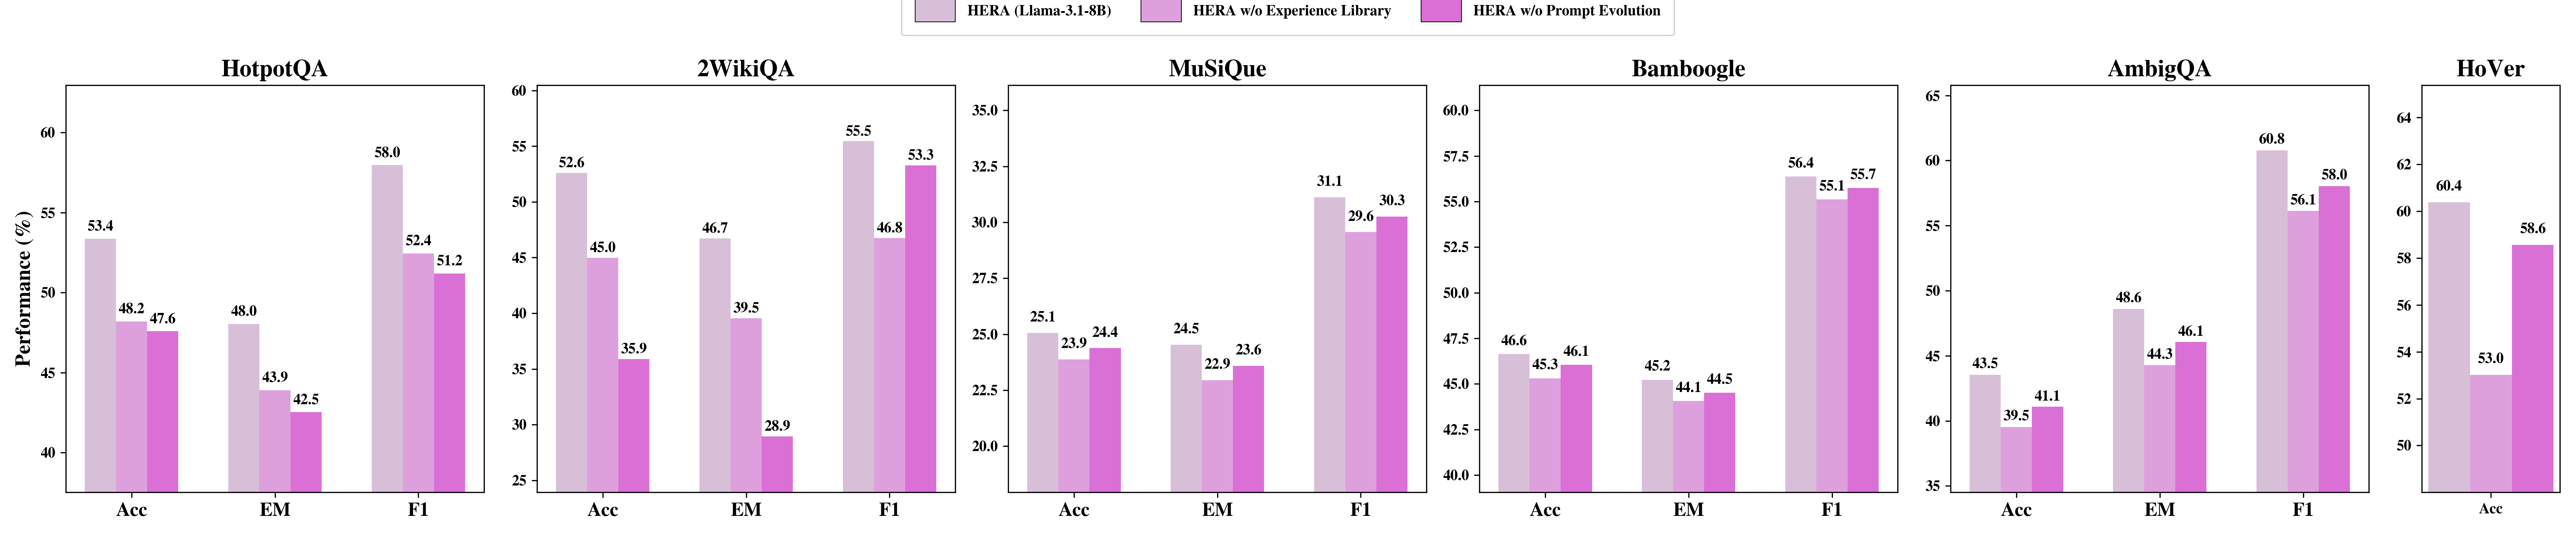
\includegraphics[width=1\linewidth]{figures/llama_per_dataset.png}
        \caption{Ablation Studies of \hero with \llama as the backbone. }
        \label{fig:abla_llama}
\end{figure}